
\chapter{System design}
	\section{System overview} \label{sec:system}

\begin{figure}[h]
    \centering
    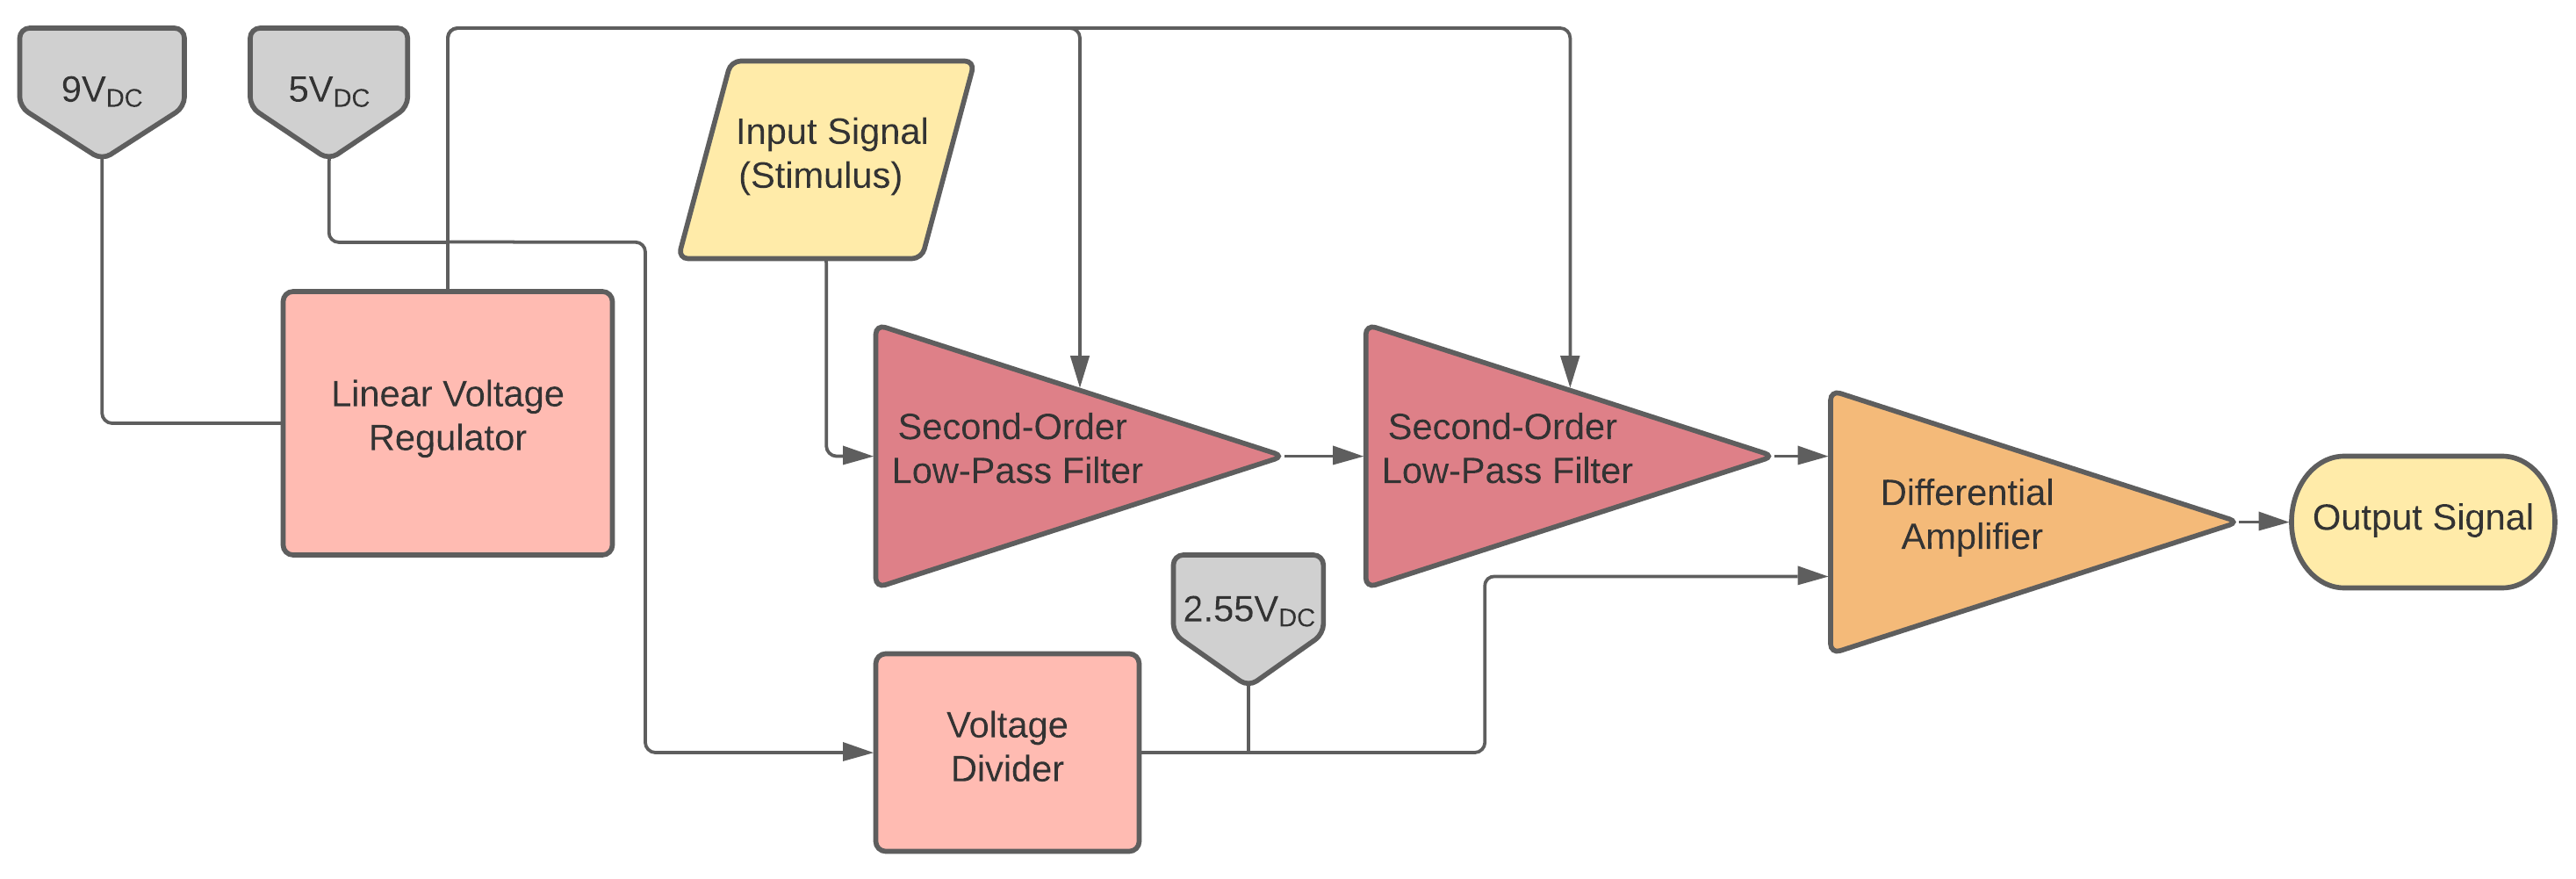
\includegraphics[width = 1\textwidth]{Figures/1.1_block}
    \caption{System Block Diagram}
    \label{fig:1.1_block}
\end{figure}

As part of the health monitoring system, which consists of an analogue temperature sensor and an optic heart rate monitor, a voltage regulation circuit is required, as well as a signal conditioning and amplification system. This report focuses on the design and implementation of the latter components. Figure \ref{fig:1.1_block} gives an overview of the combined system, where the voltage regulator supplies power to the circuital components responsible for filtering the signal, removing its offset, and then amplifying the signal which is originally received from an analog temperature sensor. Two second-order low-pass filters were cascaded to clear the signal of noise. This may seem excessive at first, but the cascaded setup allows for the use of less costly components (see Section \ref{sec:temp_design}), as well as producing an output signal subject to very low noise (see Section \ref{sec:temp_results}). Since the filtered signal still has a DC offset, and the amplifier needs a virtual ground, the voltage divider connects to the amplifier in such a way as to simultaneously remove the input DC offset and add the virtual ground. Finally, the differential amplifier increases the magnitude of the input signal to the degree needed at the input of a microcontroller ADC, which will be used to interpret the temperature sensor output. Note that this circuit design does not include a voltage buffer, as it was decided against upon noting that the desired output was easily obtained without a buffer, and omitting the buffer resulted in much lower current drawn from the battery (see Section \ref{sec:temp_design}), as well as resulting in lower total cost due to less components present in the circuit. Analysis and simulation of all circuits was done with the simulation software LTSpice.

\vfill









